Clasifica los cuerpos geométricos.
\begin{figure}[H]
    \centering
    \begin{subfigure}{.18\linewidth}
        \centering
        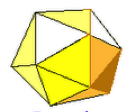
\includegraphics[width=\linewidth]{../images/sinma2_aiu3_ac79_img01}
        \caption{Clasificación:\\\fillin[poliedro][1.6cm]}
        \label{sfig:sinma2_aiu3_ac79_img01}
    \end{subfigure}\qquad
    \begin{subfigure}{.18\linewidth}
        \centering
        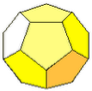
\includegraphics[width=\linewidth]{../images/sinma2_aiu3_ac79_img02}
        \caption{Clasificación:\\\fillin[poliedro][1.6cm]}
        \label{sfig:sinma2_aiu3_ac79_img02}
    \end{subfigure}\qquad
    \begin{subfigure}{.18\linewidth}
        \centering
        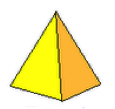
\includegraphics[width=\linewidth]{../images/sinma2_aiu3_ac79_img03}
        \caption{Clasificación:\\\fillin[pirámide][1.6cm]}
        \label{sfig:sinma2_aiu3_ac79_img03}
    \end{subfigure}
    \qquad
    \begin{subfigure}{.25\linewidth}
        \centering
        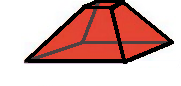
\includegraphics[width=.8\linewidth]{../images/sinma2_aiu3_ac79_img04}
        \caption{Clasificación:\\\fillin[tronco de pirámide][3.5cm]}
        \label{sfig:sinma2_aiu3_ac79_img04}
    \end{subfigure}
    \\
    \begin{subfigure}{.25\linewidth}
        \centering
        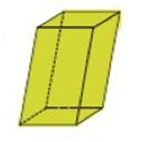
\includegraphics[width=.8\linewidth]{../images/sinma2_aiu3_ac79_img05}
        \caption{Clasificación:\\\fillin[prisma rectangular oblicuo][4.5cm]}
        \label{sfig:sinma2_aiu3_ac79_img05}
    \end{subfigure}\qquad
    \begin{subfigure}{.18\linewidth}
        \centering
        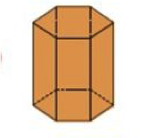
\includegraphics[width=\linewidth]{../images/sinma2_aiu3_ac79_img06}
        \caption{Clasificación:\\\fillin[prisma hexagonal][3cm]}
        \label{sfig:sinma2_aiu3_ac79_img06}
    \end{subfigure}\qquad
    \begin{subfigure}{.18\linewidth}
        \centering
        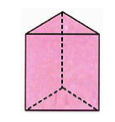
\includegraphics[width=\linewidth]{../images/sinma2_aiu3_ac79_img07}
        \caption{Clasificación:\\\fillin[prisma triangular][3cm]}
        \label{sfig:sinma2_aiu3_ac79_img07}
    \end{subfigure}\qquad
    \begin{subfigure}{.25\linewidth}
        \centering
        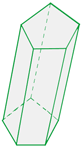
\includegraphics[width=.45\linewidth]{../images/sinma2_aiu3_ac79_img08}
        \caption{Clasificación:\\\fillin[prisma pentagonal oblicuo][4.5cm]}
        \label{sfig:sinma2_aiu3_ac79_img08}
    \end{subfigure}\qquad
    \begin{subfigure}{.18\linewidth}
        \centering
        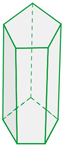
\includegraphics[width=.5\linewidth]{../images/sinma2_aiu3_ac79_img09}
        \caption{Clasificación:\\\fillin[prisma pentagonal][3cm]}
        \label{sfig:sinma2_aiu3_ac79_img09}
    \end{subfigure}
    \qquad
    \begin{subfigure}{.18\linewidth}
        \centering
        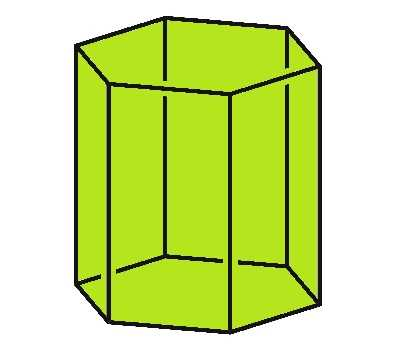
\includegraphics[width=\linewidth]{../images/sinma2_aiu3_ac79_img10}
        \caption{Clasificación:\\\fillin[prisma heptagonal][3cm]}
        \label{sfig:sinma2_aiu3_ac79_img10}
    \end{subfigure}
    \caption{Cuerpos geométricos}
    \label{fig:figuras_geo3d}
\end{figure}

% \begin{multicols}{2}
%     \centering
%     \fbox{
%         \begin{minipage}[t]{0.8\linewidth}
%             Prisma recto \vspace{6cm}
%         \end{minipage}
%     }\columnbreak
%     \fbox{
%         \begin{minipage}[t]{0.8\linewidth}
%             Otro \vspace{6cm}
%         \end{minipage}
%     }
% \end{multicols}
